\section{Umsetzung}

\begin{itemize}
	\item Ausgewählte Implementierungsdetails (Bsp. Algorithmen, Datenstrukturen, Libraries, Architectural Hot Spots)Dokumentation Architektur und Design (i.d.R. plattformneutral bzw. technologieübergreifend, z.B. in Form von UML-Diagrammen und Erläuterungen dazu)
	\item Dokumentation, welche Experimente/Tests durchgeführt wurden und welche Lösungsoptionen aufgrund der Ergebnisse dieser Experimente/Tests verworfen wurden.
\end{itemize}

\subsection{Labor Netzwerk Architektur} \label{subsec:Labor-Netzwerk-Architektur}
Mit der zur Verfügung gestellten Hardware ist die folgende Netzwerk Architektur entstanden.

Folgende zentrale Überlegungen sind eingeflossen:

\begin{itemize}
	\item Campus Netzwerk mit mehreren Gebäuden, um das Wandern von Geräten zu simulieren.
	\item Mischung der zur Verfügung stehenden Switches (Catalyst 9300 \& 3850) in der Fabric Edge Nodes, um Verhalten zu vergleichen.
	\item Management Netzwerk ist inbound. Kabelführung zu jedem Switch ist meistens von den Gegebenheiten in typsichen Gebäuden nicht möglich.
\end{itemize}


\begin{figure}[H]
	\centering
	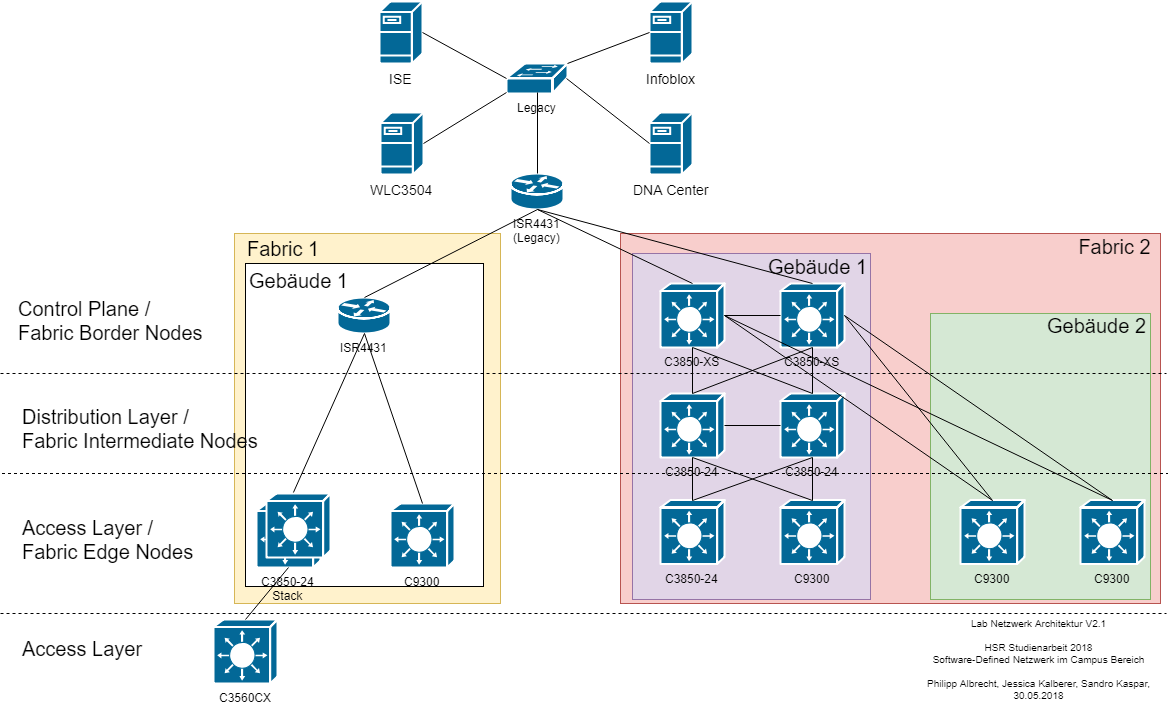
\includegraphics[width=1\linewidth]{img/LabNetworkArchitecture.png}\\[1px]
	\caption{SDN Netzwerk Architektur}
	\label{fig:LabNetworkArchitecture}
\end{figure}

\subsection{Netzwerkarchitekturen Vergleich}
Hauptunterschiede zwischen der klassischen Netzwerkarchitektur und der "Modernen" Software-Defined Access Architektur. 

\begin{itemize}
	\item Bis zur Fabric Edge Nodes (Vergleichbar mit dem Access Layer) unterliegt ein Layer 3 Netzwerk. 
	\item Kein Einsatz von STP oder VSS auf Distribution Layer notwendig, da das Underlay Netzwerk rein Layer 3 ist und Routing Protokolle (OSPF) zum Einsatz kommen.
	\item Der Distribution Layer nimmt neu als Fabric Intermediate Nodes nur noch die Funktion als Layer 3 Brücke bzw. VXLAN transporteuer ein, anstatt die Grenze zwischen Layer 3 und Layer 2 zu sein. Die Fabric Intermediate Nodes sind optional. 
	\item Während beim klassischen Design die logische Netzwerkarchitektur direkt Abhängig ist von der physikalischen Architektur, wird bei SDN die phykalische Netzwerkarchitektur von der logischen Architektur getrennt. Man spricht dann von der Physical Fabric Topology bzw. Underlay und den entsprechenden Layer 2 bzw. Layer 3 Overlay Network. 
\end{itemize}

\begin{figure}[H]
	\centering
	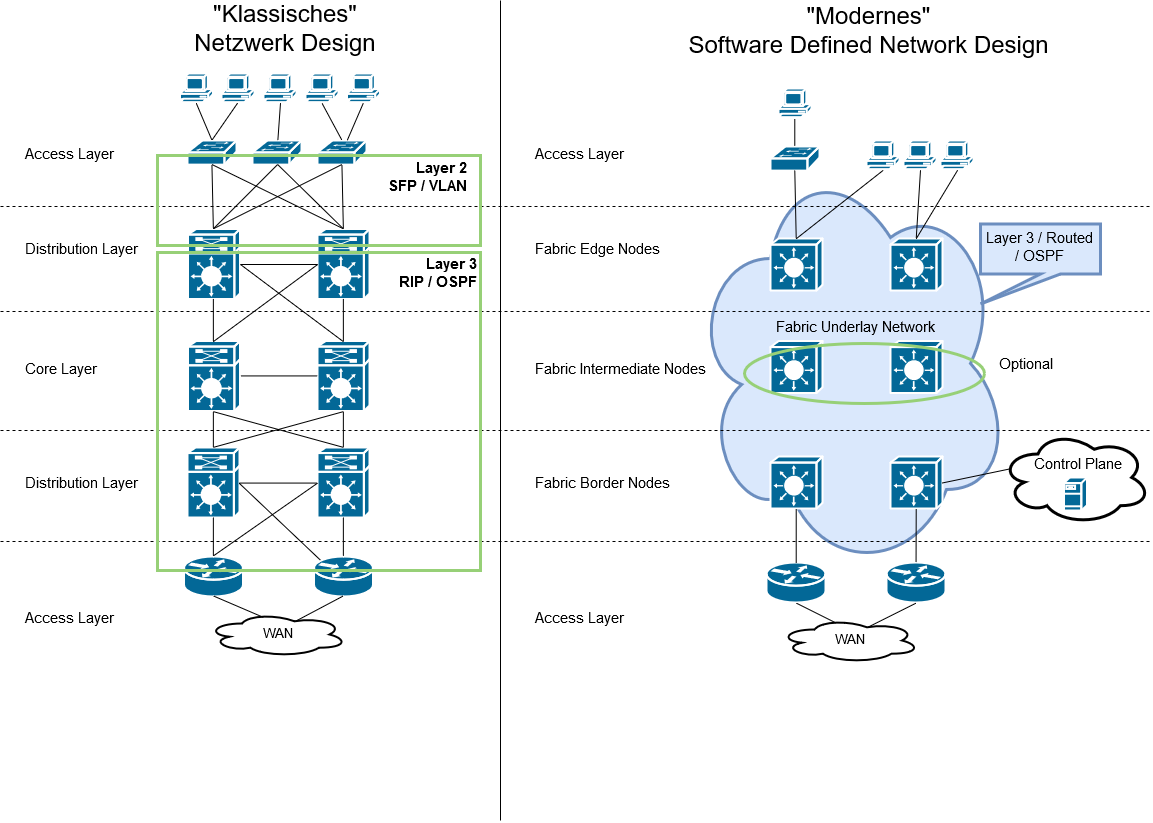
\includegraphics[width=1\linewidth]{img/LabNetworkArchitecture_Vergleich.png}\\[1px]
	\caption{Netzwerk Architektur Vergleich}
	\label{fig:LabNetworkArchitectureVergleich}
\end{figure}

\subsection{Maximale Skalierungen}
Nachfolgend werden die aktuell maximalen Skalierungen des DNA Centers, sowie der Border und Edge Nodes aufgelistet.
\begin{figure}[H]
	\centering
	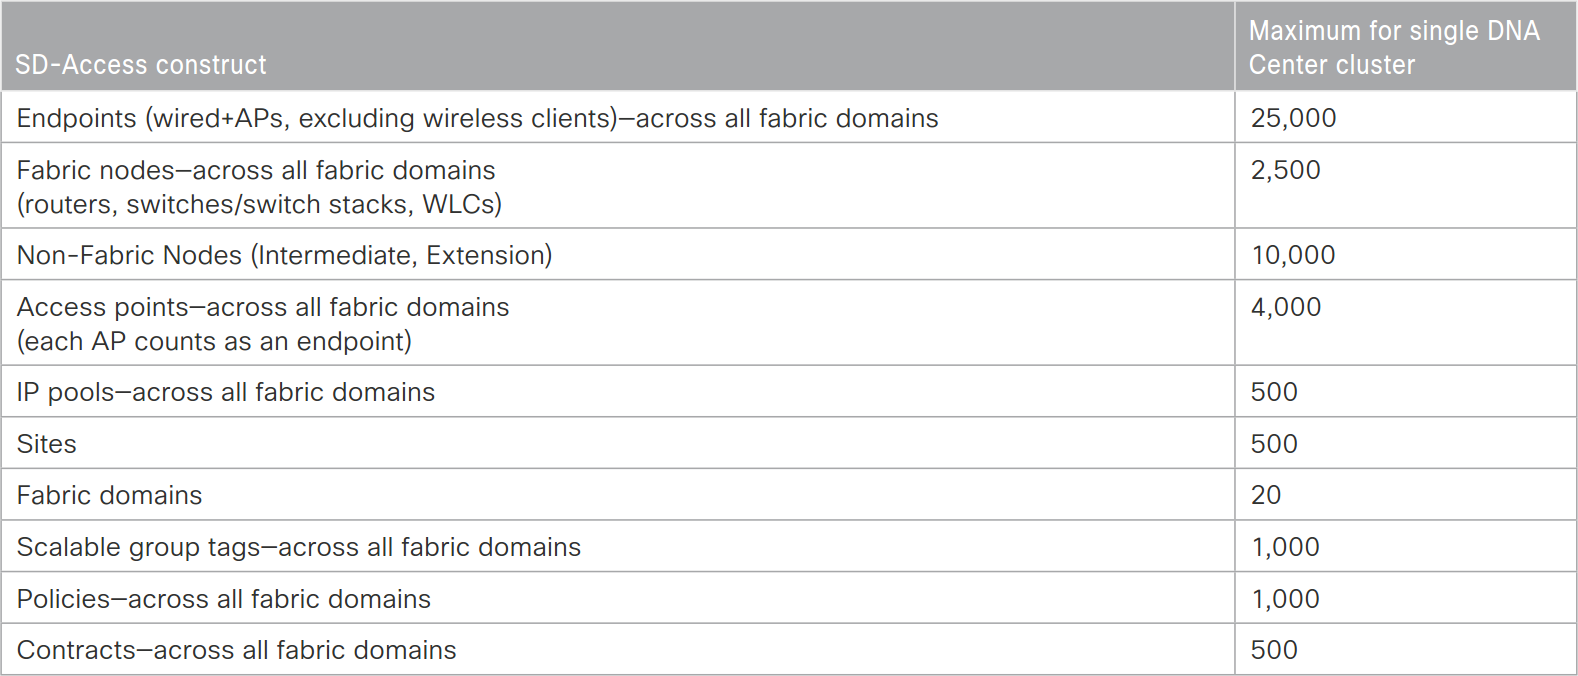
\includegraphics[width=1\linewidth]{img/MaximumScale-HACluster.png}\\[1px]
	\caption{DNA Center Maximum Scale Constraints HA Cluster}
	\label{fig:Maximum Scale HACluster}
\end{figure}

\begin{figure}[H]
	\centering
	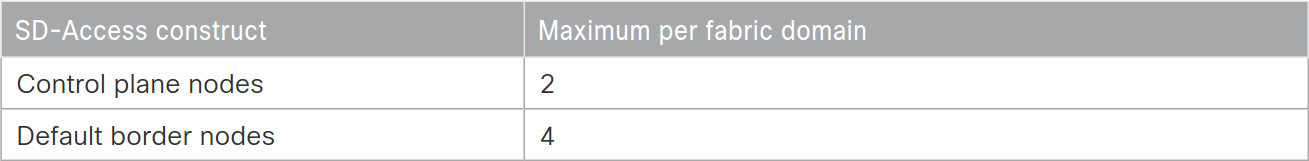
\includegraphics[width=1\linewidth]{img/MaximumScale-Fabric.png}\\[1px]
	\caption{DNA Center Maximum Scale Constraints Fabric}
	\label{fig:Maximum Scale Fabric}
\end{figure}

\begin{figure}[H]
	\centering
	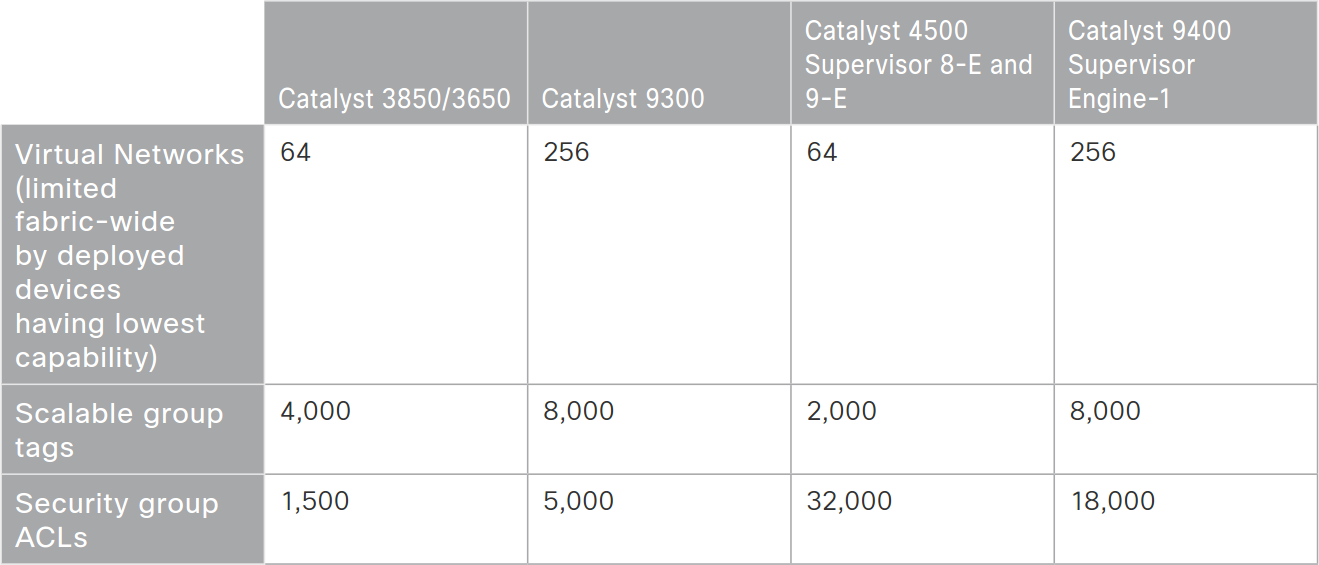
\includegraphics[width=1\linewidth]{img/MaximumScale-EdgeNode.png}\\[1px]
	\caption{SDA Edge Node Scale Constraints}
	\label{fig:SDA Edge Node Scale Constraints}
\end{figure}

\begin{figure}[H]
	\centering
	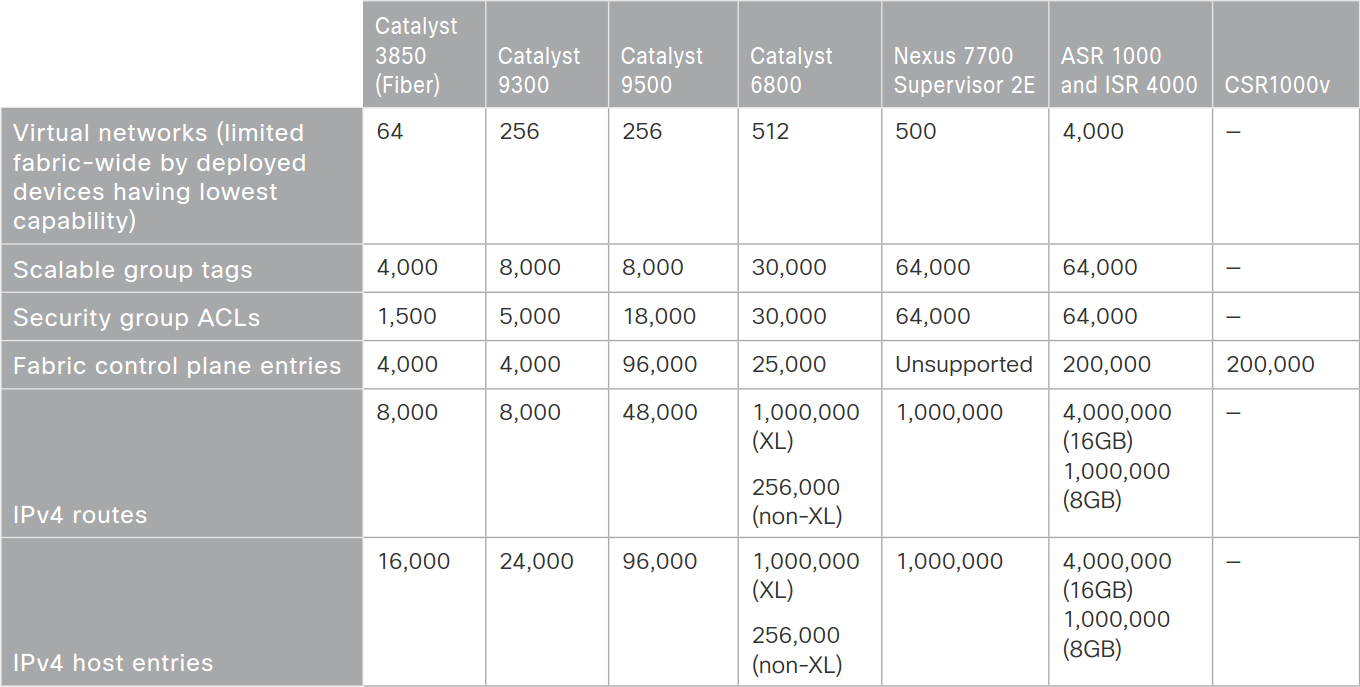
\includegraphics[width=1\linewidth]{img/MaximumScale-BorderNode.png}\\[1px]
	\caption{SDA Border Node Scale Constraints}
	\label{fig:SDA Border Node Scale Constraints}
\end{figure}

\pagebreak
\subsection{Verkabelungsplan}
Auf nachfolgendem Verkabelungsplan sind die genauen Ports zwischen den Geräten ersichtlich, so dass für Konfigurationen die richtigen Interfaces schnell gefunden werden können.
\begin{figure}[H]
	\centering
	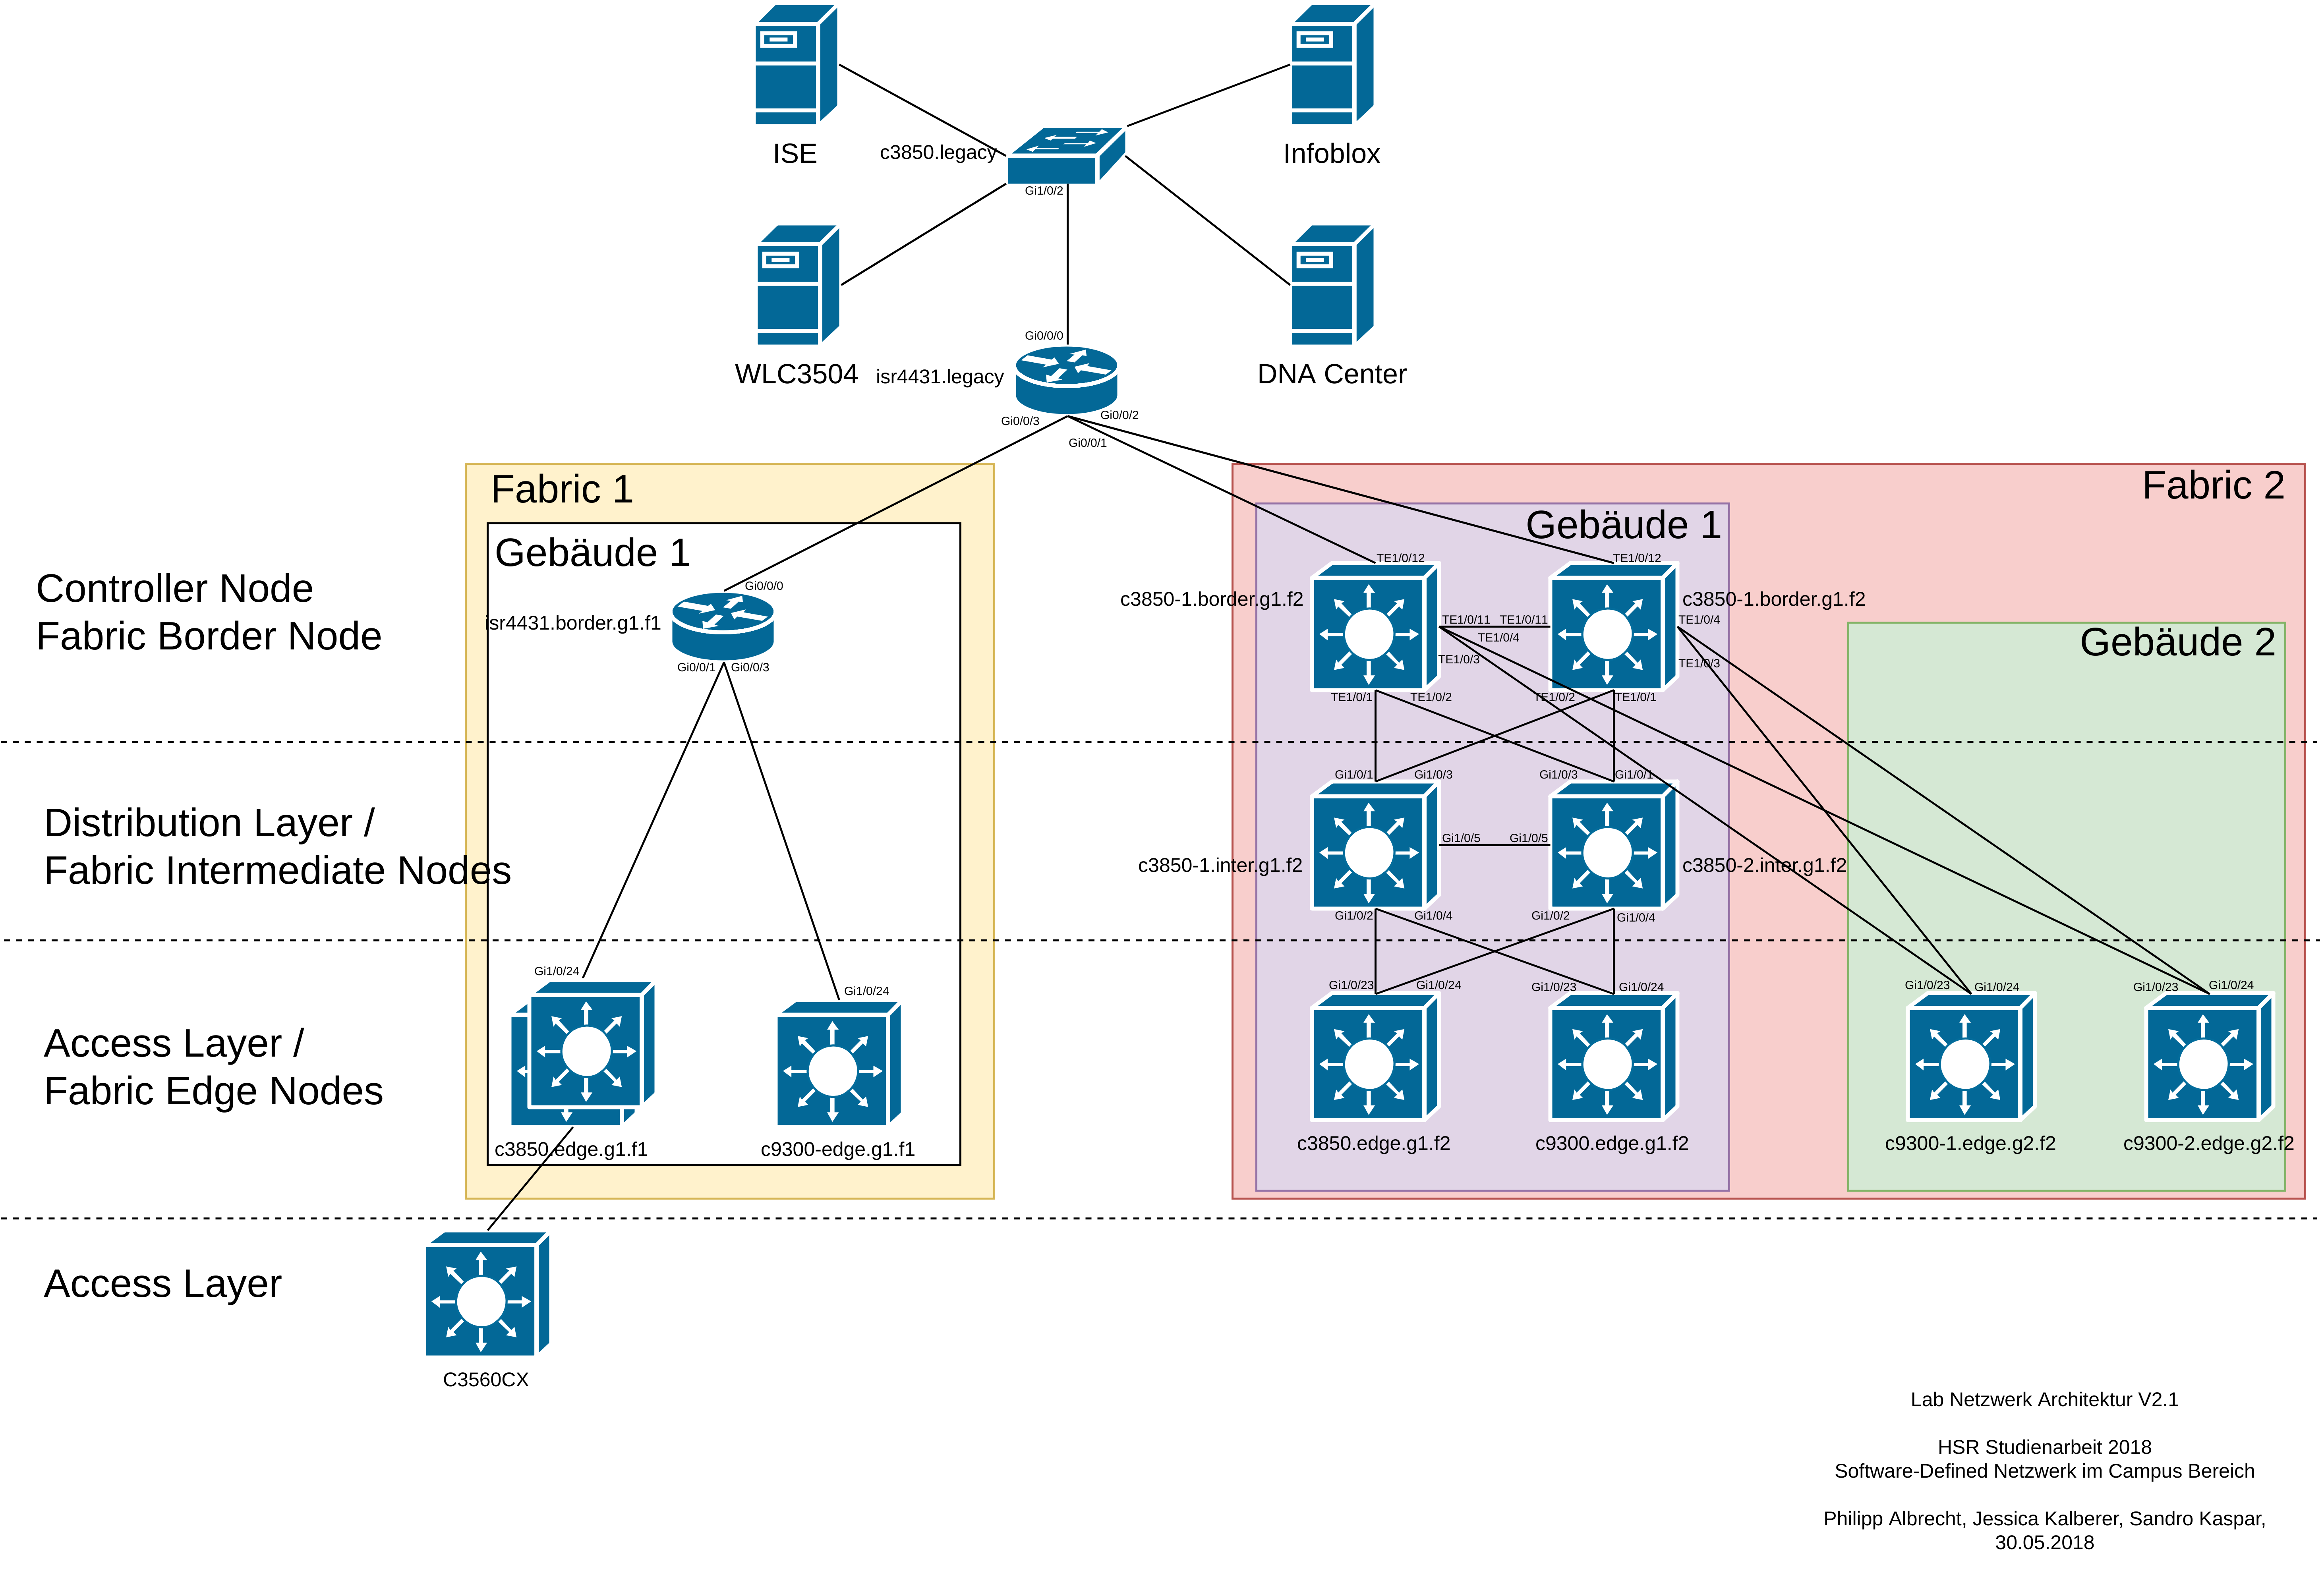
\includegraphics[angle=90,width=0.9\linewidth]{img/LabNetworkArchitecture-Interfaces.png}\\[1px]
	\caption{Lab Architecture with physical Interfaces}
	\label{fig:Lab Architecture with physical Interfaces}
\end{figure}


